%
% mandeljulia.tex -- Mandelbrot/Julia
%
% (c) 2021 Prof Dr Andreas Müller, OST Ostschweizer Fachhochschule
%
\bgroup
\def\l{3}
\pgfmathparse{\l/50}
\xdef\u{\pgfmathresult}
\def\gitter#1{
	\foreach \x in {-50,-40,...,50}{
		\draw[line width=0.1pt,color=#1]
			({\x*\u},-\l) -- ++(0,{2*\l});
		\draw[line width=0.1pt,color=#1]
			(-\l,{\x*\u}) -- ++({2*\l},0);
	}
}
\pgfmathparse{40*\u}
\xdef\s{\pgfmathresult}
\def\punkt#1#2{
	({(#1)*\s+20*\u},{(#2)*\s+0})
}
\def\achsen#1{
	\draw[->,color=#1] \punkt{-1.8}{0} -- \punkt{0.9}{0}
		coordinate[label={$\operatorname{Re}$}];
	\draw[->,color=#1] \punkt{0}{-1.3} -- \punkt{0}{1.4}
		coordinate[label={right:$\operatorname{Im}$}];
	\draw[color=#1] \punkt{-1}{0} -- ++(0,0.1);
	\draw[color=#1] \punkt{-1}{0} -- ++(0,-0.1);
	\draw[color=#1] \punkt{0.5}{0} -- ++(0,0.1);
	\draw[color=#1] \punkt{0.5}{0} -- ++(0,-0.1);
	\draw[color=#1] \punkt{0}{1} -- ++(0.1,0);
	\draw[color=#1] \punkt{0}{1} -- ++(-0.1,0);
	\draw[color=#1] \punkt{0}{-1} -- ++(0.1,0);
	\draw[color=#1] \punkt{0}{-1} -- ++(-0.1,0);
	\node[color=#1] at \punkt{-1}{0} [below left] {$-1$};
	\node[color=#1] at \punkt{0}{-1} [below left] {$-1$};
	\node[color=#1] at \punkt{0}{1} [above left] {$1$};
	\node[color=#1] at \punkt{0.5}{0} [below right] {$\frac12$};
}
\begin{frame}[t]
\setlength{\abovedisplayskip}{5pt}
\setlength{\belowdisplayskip}{5pt}
\frametitle{Mandelbrot-Menge/Julia-Menge}
\begin{center}
\vspace*{-10pt}
\begin{tikzpicture}[>=latex,thick]

\begin{scope}[xshift=-3.4cm]
	\node at (0,-3) [below] {Parameter-Raum\strut};
	\achsen{black}
	\begin{scope}
		\clip (-\l,-\l) rectangle (\l,\l);
		\node at (-0.59,-0.32) {
\includegraphics[width=11.2cm]{../slides/1/mandelbrot.jpg}};
		\achsen{white}
	\end{scope}
	\uncover<2->{
		\gitter{white}
	}
	\uncover<3->{
		\fill[color=white] \punkt{-0.47}{0.45} circle[radius=0.08];
		\node[color=white] at \punkt{-0.47}{0.45}
			[above left] {$-0.47+0.45i$};
	}
\end{scope}

\begin{scope}[xshift=3.4cm]
	\only<4>{
		\node at (0,0) {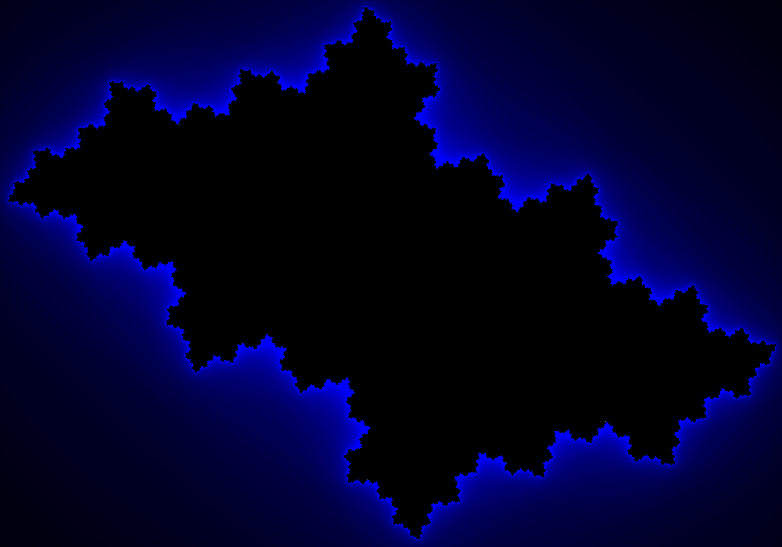
\includegraphics[width=6cm]{../slides/1/einzelne_julia_menge.png}};
	}
	\only<5>{
		\node at \punkt{-0.47}{0.45}
		{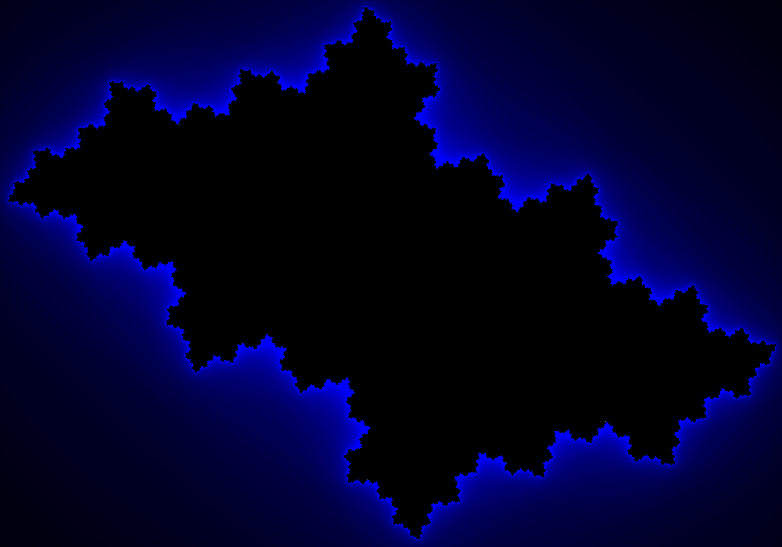
\includegraphics[width=5.0cm]{../slides/1/einzelne_julia_menge.png}};
	}
	\only<6>{
		\node at \punkt{-0.47}{0.45}
		{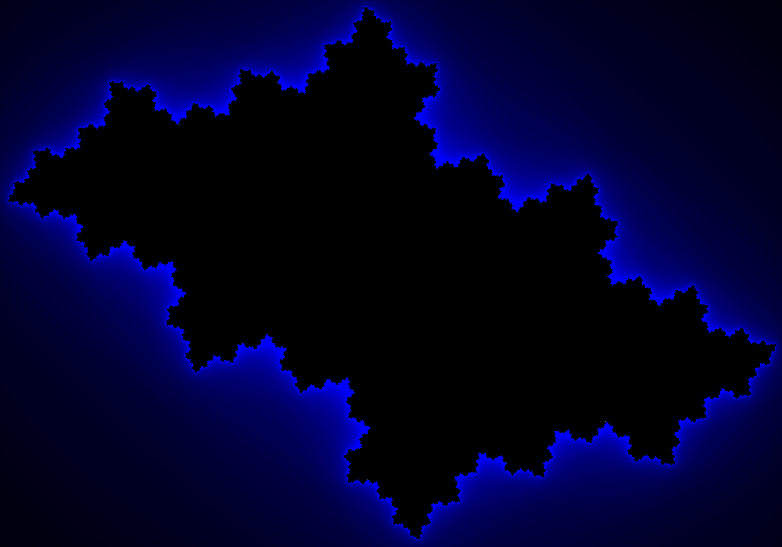
\includegraphics[width=4.0cm]{../slides/1/einzelne_julia_menge.png}};
	}
	\only<7>{
		\node at \punkt{-0.47}{0.45}
		{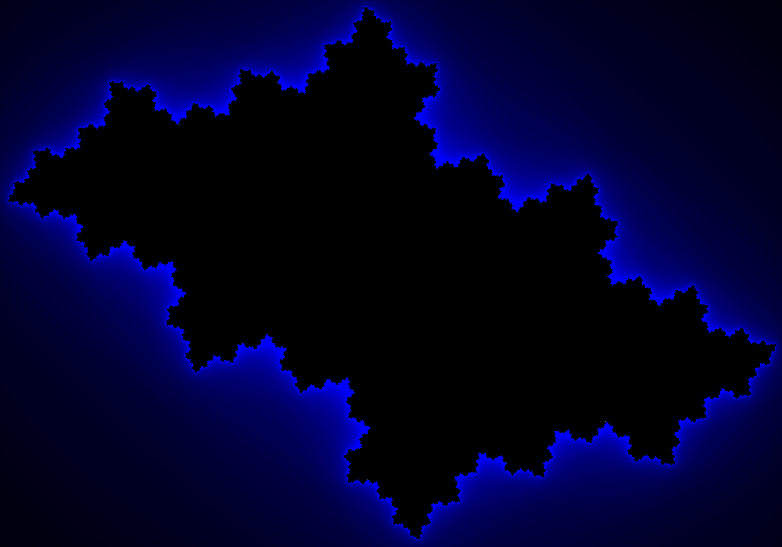
\includegraphics[width=3.0cm]{../slides/1/einzelne_julia_menge.png}};
	}
	\only<8>{
		\node at \punkt{-0.47}{0.45}
		{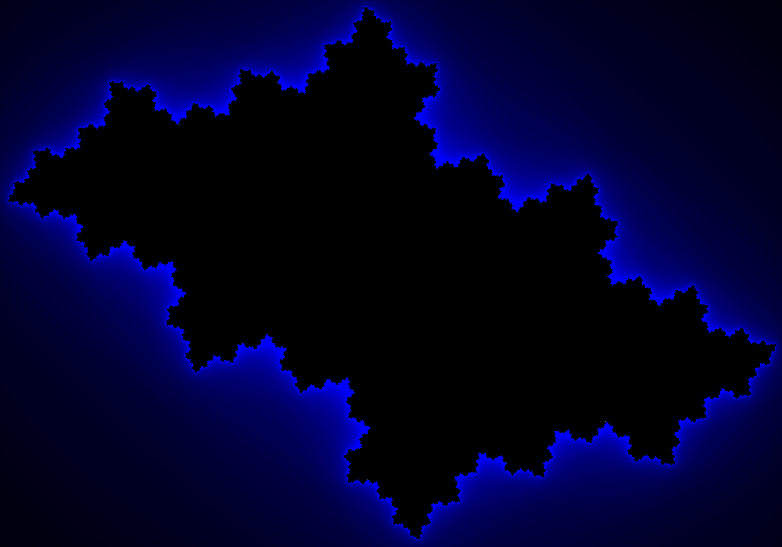
\includegraphics[width=2.0cm]{../slides/1/einzelne_julia_menge.png}};
	}
	\only<9>{
		\node at \punkt{-0.47}{0.45}
		{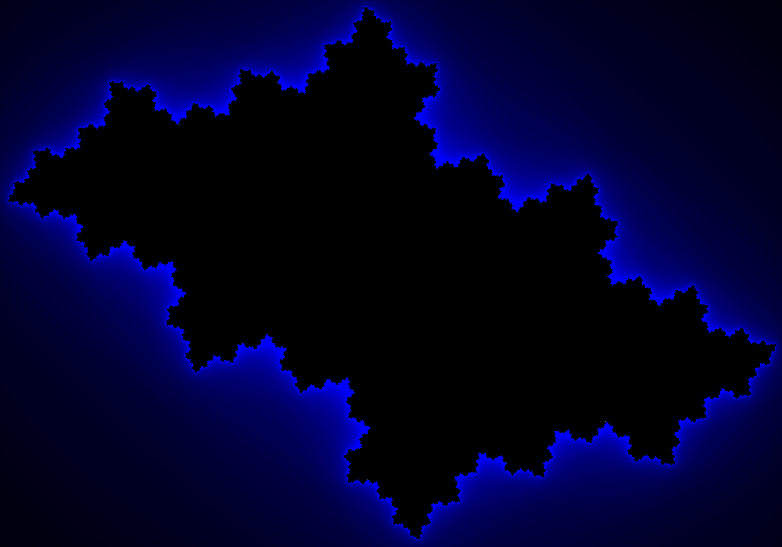
\includegraphics[width=1.0cm]{../slides/1/einzelne_julia_menge.png}};
	}
	\only<10>{
		\node at \punkt{-0.47}{0.45}
		{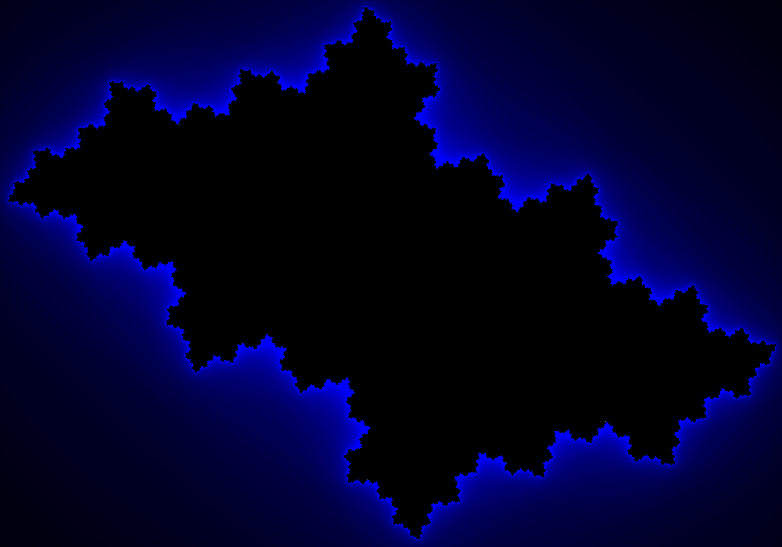
\includegraphics[width=0.5cm]{../slides/1/einzelne_julia_menge.png}};
	}
	\only<11>{
		\node at \punkt{-0.47}{0.45}
		{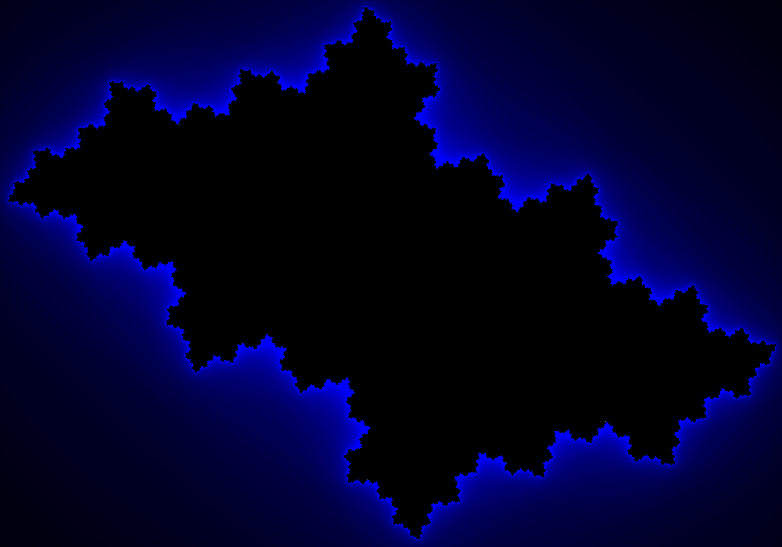
\includegraphics[width=0.2cm]{../slides/1/einzelne_julia_menge.png}};
		
	}
	\uncover<5->{
		\achsen{black}
	}
	\uncover<12>{
		\node at (0,0) {
\includegraphics[width=6cm]{../slides/1/julia_mosaik_scaled.jpg}};
		\begin{scope}
			\clip (-\l,-\l) rectangle (\l,\l);
			\achsen{white}
		\end{scope}
	}
	\uncover<5-11>{
		\gitter{gray}
	}
	\uncover<12>{
		\gitter{white}
		\draw[color=white]
			\punkt{(-0.47-0.01)}{(0.45-0.01)}
			rectangle
			\punkt{(-0.47+0.01)}{(0.45+0.01)};
		\node[color=white] at \punkt{-0.47}{0.45}
			[above left] {$-0.47+0.45i$};
	}
	\uncover<1-4>{
		\node at (0,-3) [below] {Zustands-Raum\strut};
	}
	\foreach \n in {5,...,12}{
		\pgfmathparse{(\n-5)/7}
		\xdef\t{\pgfmathresult}
		\only<\n>{
			\node[opacity={1-\t}] at (0,-3)
				[below] {Zustands-Raum\strut};
			\node[opacity={\t}] at (0,-3)
				[below] {Parameter-Raum\strut};
		}
	}
\end{scope}

\end{tikzpicture}
\end{center}
\end{frame}
\egroup
